% !TeX root = 00_nesting_paper-short.tex



%We now want to focus on a specific instance of the problem stated in Algorithm \ref{alg:general}: suppose to store a graph using adjacency lists \texttt{[similarly to the one proposed in the Graph Join algorithm]}; in particular,  The main data structure over which this algorithm relies  is presented in Figure \ref{nestedGraphVertex}: it shows that minor changes have been applied to the original data structure that was used to serialize graph within the graph join scenario. %Moreover, in this case we mark with different hash values the vertices within the data structure satisfying different predicates within the predicates. 
%Given that the data structure requires a simple linear visit of the graph, no additional primary and secondary data structures are required. 
%Nevertheless, during our serialization phase we provide both a primary index for accessing external informations (\textit{VertexIndex}) and the serialization of all the vertices' adjacency lists, which is going to be used for traversing the graph (\textit{VertexVals}). 
%%In our  implementation, hash values are here used only as placeholders for the nodes' labels used within the patterns.
%but, given that vertices are not sorted by hash value as for graph joins, we keep the hash fields for both backward compatibility and in order to make graph joins possible for nested graphs, too.

\begin{figure*}[!ht]
	\centering
	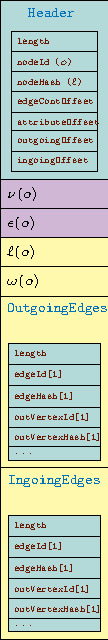
\includegraphics[height=.7\textheight,angle =90]{test}
	\caption{Serialized data structure representing an extended adjacency list for one nested vertex $o$. The header contains some basic information (such the representation size of $o$, its id and associated hash) and the offsets to the remaining fields. $\nu$ and $\epsilon$ are empty when the serialized graph represents a basic property graph as the one in Figure \ref{fig:inputbibex2}.}\label{nestedGraphVertex}
\end{figure*}
\section{Graph Nesting}\label{sec:nestingdef}
The graph nesting operator uses a classifier to group all the vertices and edges that shall appear as a member of a cluster $C$. 

\begin{definition}[Nested Graph Classifier, $g_\kappa$]
	Given a set of cluster labels $\mathcal{C}$, a \textbf{nested graph classifier} operator $g_\kappa$ maps a nested property graph $G_o$ into a nested property graph collection $\{G_C\}_{C\in\mathcal{C},G_C\neq \emptyset}$ of subgraphs of $G_o$. Such operator uses a classifier function $\kappa\colon \VS\cup \ES\to \wp(\mathcal{C})$ mapping each vertex or edge in either no graph or more than one non-empty subgraph. Each nested graph $G_C$ is a pair
	$G_C=\Braket{\VS_C,\ES_C}$
	where $\VS_C$ (and $\ES_C$) is the set of all the vertices $v$ (and edges $e$) in $G_o$ having $C\in \kappa(v)$ (and $C\in \kappa(e)$). Therefore, the nested graph classifier is defined as follows:
	\[g_\kappa(G_o)=\Set{\Braket{\VS_C,\ES_C}|C\in\mathcal{C},\VS_C\neq\emptyset,\ES_C\neq\emptyset}\]
\end{definition}

The former definition is also going to express graph pattern evaluations, where $\kappa$ may be represented as a graph (cf. Neo4J). In order to represent the subgraphs in $g_\kappa(G_o)$ as either vertices and edges, we may use
the following \textsc{User-Defined Functions}:
\begin{definition}[User-Defined Functions]
	An \textbf{object user defined function} $\mu_\Omega$ maps each subgraph $G_C\in g_\kappa(G_o)$ into a pair $\mu_\Omega(G_C)=(L,t)$, where $L\in\wp(\Sigma^*)$ is a set of labels and $t$ is a relational tuple.
	
	An \textbf{edge user defined function} $\mu_E$ maps each subgraph $G_C\in g_\kappa(G_o)$ into a pair of identifiers $\mu_E(G_C)=(s,t)$ where $s,t\in\mathbb{N}^2$.
\end{definition}

While $\mu_\Omega$ may be used for transforming subgraphs to both vertices and edges, $\mu_E$ is only used to map subgraphs to edges. In order to complete such transformation,  we have to map each graph in $g_\kappa(G)$ into a new id $(\textbf{c},\textbf{i})\notin \VS\cup \ES$, for which an indexing function has to be defined as follows:
\[\iota_G(G_C)=(\max\Set{c|(c,i)\in V\cup E}+1,dt(\mathcal{V}_C\cup \mathcal{E}_C))\]
where $dt$ is an arbitrary bijection associating a  $n$-tuple in $\mathbb{N}^n$ to one single number $\mathbb{N}$ \cite{odifreddi1992}. The combination of all the previous functions allow the definition of the following nesting operator:



\begin{definition}[Graph Nesting]
	Given a nested graph $G_{(c,i)}$ within a nested graph database $G$, an object user defined function $\mu_\Omega$, an edge user defined function $\mu_E$ and an indexing function $\iota_G$,
	the graph nesting operator $\eta_{g_V,g_E,\mu_\Omega,\mu_E,\iota_G}^{\textbf{keep}}$ converts each subgraph in $G_C\in g_V(G_{(c,i)})$ (and $G_C\in g_E(G_{(c,i)})$) into a nested vertex (and nested edge) $\iota_G(G_C)$ and adds them in a nested vertex $(\overline{c},i):=(\max\{c|(c,i)\in(V\cup E)\}+1,i)$, to which the following nested graph is associated:
	\[\begin{split}
	\eta&{}_{g_V,g_E,\mu_\Omega,\mu_E,\iota_G}^{\textbf{keep}}(G_{(c,i)})=G_{(\overline{c},i)}\\
	\end{split}\]
	The vertices and edges in $G_{(c,i)}$ that appear neither in a nested vertex nor in a nested edge may be also returned if $\textbf{keep}$ is set to \texttt{true}. As a result, the nested graph database is updated by using the nested graph classifier and user defined functions as follows:
	\[\begin{split}
	\Big\langle&\VS\cup \iota_G(g_V(G_{(c,i)}))\cup\{(\overline{c},i)\}, \ES\cup \iota_G(g_E(G_{(c,i)})),\\
	& \lambda\oplus \bigoplus_{G_C\in g_E(G_{(c,i)})}\iota_G(G_C)\mapsto \mu_E(G_C),\\
	& \ell\oplus\bigoplus_{G_C\in g_E(G_{(c,i)})\cup g_V(G_{(c,i)})}\iota_G(G_C)\mapsto\texttt{fst}\;\mu_\Omega(G_C),\\
	& \omega\oplus\bigoplus_{G_C\in g_E(G_{(c,i)})\cup g_V(G_{(c,i)})}\iota_G(G_C)\mapsto\texttt{snd}\;\mu_\Omega(G_C),\\
	& \nu\oplus \bigoplus_{G_C\in g_E(G_{(c,i)})\cup g_V(G_{(c,i)})}\iota_G(G_C)\mapsto V_C\\
	& \;\; \oplus (\overline{c},i)\mapsto \{v\in \nu(c,i) | V(v)=\emptyset\wedge\textbf{keep} \}\cup \iota_G(g_V(G_{(c,i)})) \\
	& \epsilon\oplus \bigoplus_{G_C\in g_E(G_{(c,i)})\cup g_V(G_{(c,i)})}\iota_G(G_C)\mapsto E_C\Big\rangle\\
	& \;\; \oplus (\overline{c},i)\mapsto\{e\in \epsilon(c,i) | E(e)=\emptyset\wedge\textbf{keep} \}\cup \iota_G(g_E(G_{(c,i)}))\Big\rangle
	\end{split}\]
	where $f\oplus g$ denotes the extension of the (finite) function $f$ with another (finite) function $g$. $a\mapsto b$ defines a finite function, which domain contains only $a$.
\end{definition}


\section{Two HOp Separated Patterns Algorithm}
\label{sec:THOSPA}
In order to solve our specific graph nesting problem as presented in the introduction, we want to evaluate $\eta$ when the non-traversed vertices and edges are not preserved ($\textbf{keep}=\texttt{false}$), where $g_V$ and $g_E$ are the ones represented in Figure \ref{fig:bibex2} and the UDFs associate to each nested vertex the authors' informations and creates nested edges with \texttt{coAuthorship} label and no associated tuple. In particular:
\[\begin{split}
\mu_E(G_C)&=\Braket{(\overline{c},\texttt{snd}f_C(\gamma_E^{src})),(\overline{c},\texttt{snd}f_C(\gamma_E^{dst}))}\; s.t.\\
&\; g_E\xrightarrow{f_C}G_C,\quad \overline{c}=\max\{c|(c,i)\in\mathcal{V}\cup\mathcal{E}\}+1\\
\end{split}\]
\[\mu_\Omega(G_C)=\begin{cases}
([\mstr{coAuthor}],\;\emptyset) & G_C \in g_E(G_{(c,i)})\\
(\ell(f_C(\gamma_V))),\;\omega(f_C(\gamma_V))) & G_C \in g_V(G_{(c,i)})\\
\end{cases}\]


The \textbf{input data  represnetation} for the THoSP algorithm is presented in Figure \ref{nestedGraphVertex}, which represents an  extension of the usual graph adjacency lists. In addition to the information pertaining to both the ingoing and outgoing edges, each vertex $o$ has an associated \texttt{header} containing its id ($o$), its associated hash and the offset pointing to other serialzied fields, such as the information of the  nested vertices and edges a set of labels ($\ell(o)$), and eventually its property-value representation ($\omega(o)$). Last, for each edge we store its id and hash value, as well as the hash and the id of the adjacent vertex. Hash values are used within the proposed THoSP algorithm to store the correspondences with the graph patterns in Figure \ref{fig:patterns}; therefore, each $h(o)\approx \ell(o)$ is associated to a distinct hash value. We also suppose that the input graph data to be serialized does not represent an exact adjacency list: for this reason, the graph is firstly created in primary memory without the offset information, and then serialized into secondary memory. This first preprocessing step provides the loading and indexing step of our algorithm, where no further ancillary indexing data structures are serialized.









%\begin{table*}[!t]
%	\centering
%	\begin{tabular}{@{}cr|rr@{}}
%		\toprule
%		{\textbf{Operands' Vertices}} & Matched Graphs  & {\textbf{General Nesting} (ms)} & {\textbf{THoSP} (ms)}  \\	
%		\midrule
%		$10$ & $3$ &  0.57       & 0.11\\
%		$10^2$ & $58$  & 0.73        & 0.14\\
%		$10^3$  & $968$  & 2.78   & 0.46\\
%		$10^4$ & $8,683$   & 152.11   & 4.07\\
%		$10^5$ & $88,885$   & 14,015.00 & 43.81 \\
%		$10^6$  & $902,020$  &  1,579,190.00      & 563.02\\
%		$10^7$ & $8,991,417$   &  $>$1H      & 8,202.93\\
%		$10^8$ & $89,146,891$   &  $>$1H      & 91,834.20\\
%		\bottomrule
%	\end{tabular}
%	%\end{minipage}
%	\caption{Comparing the performances of the THoSP algorithm with the naive General Nesting algorithm. This comparison shows that the previously defined algorithm has a worse performance than the THoSP one. }
%	\label{tab:comparisonTwo}
%\end{table*}


%The main data structure over which this algorithm relies  is presented in Figure \ref{nestedGraphVertex}: it shows that minor changes have been applied to the original data structure that was used to serialize graph within the graph join scenario. %%Moreover, in this case we mark with different hash values the vertices within the data structure satisfying different predicates within the predicates. 
%Given that the data structure requires a simple linear visit of the graph, no additional primary and secondary data structures are required. Nevertheless, during our serialization phase we provide both a primary index for accessing external informations (\textit{VertexIndex}) and the serialization of all the vertices' adjacency lists, which is going to be used for traversing the graph (\textit{VertexVals}). In our straightforward implementation, hash values are here used only as placeholders for the nodes' labels used within the patterns but, given that vertices are not sorted by hash value as for graph joins, we keep the hash fields for both backward compatibility and in order to make graph joins possible for nested graphs, too.

\begin{algorithm}[!t]
	\caption{Two HOp Separated Patterns Algorithm (THoSP)}\label{alg:THoSPAlgorithm}
	\begin{adjustbox}{max width=\textwidth}
		\begin{minipage}{1.2\linewidth}
			\algrenewcommand\algorithmicindent{1em}
			\begin{algorithmic}[1]
				\Procedure{PartitionHashJoin}{$(g_V,\gamma_V),({g_E},\gamma_E^{src},\gamma_E^{dst});\; \nested$}
				\State \textsc{File} $AdjFile$ = \textsc{Open\_MemoryMap}($\nested$);\label{openMMAP}
				\State \textsc{File} $Nesting$ = \textsc{Open}(\textbf{new});
				\State \textsc{Adjacency} $toSerialize$ = \par \textbf{new} \textsc{Map<Vertex,<Edge,Vertex>>}();
				\State {$\alpha:=g_V\cap {g_E}\backslash(\gamma_V\cup\gamma_E^{src}\cup\gamma_E^{dst})$;}\label{restriction}
				\For{\textbf{each vertex} $(c,v)$ in $AdjFile$}\label{firstJoin}
				\If{$(c,v)\vDash\alpha$}\label{vdashalpha}
				\For {\textbf{each} $ ((c',u),e,(c,v))\vDash \gamma_V$} \label{substantiallyIs}
				\State{$u':=(\overline{c},u)$} 
				\State{$NestingIndex$.write($\Braket{u',(c',u)}$)} 
				\State{$NestingIndex$.write($\Braket{u',e}$)}
				\State{$NestingIndex$.write($\Braket{u',(c,v)}$)}
				\For {\textbf{each} $ ((c'',w),e,(c,v))\vDash \gamma_V$} \label{substantiallyIs2}
				\If{$ ((c',u),e,(c,v),e',(c'',w))\vDash\gamma_E$}\label{thereIsEdge}
				\State{$w':=(\overline{c},w)$} 
				\State{$\varepsilon:=(\overline{c},dt(u,w))$}
				\State{$NestingIndex$.write($\Braket{\varepsilon,u}$,$\Braket{\varepsilon,e}$,$\Braket{\varepsilon,w}$,$\Braket{\varepsilon,e'}$,$\Braket{\varepsilon,v}$)} 
				\State{$toSerialize$.put($u'$,$\Braket{\varepsilon,w'}$)}
				\EndIf
				\EndFor
				\EndFor
				\EndIf
				\EndFor
				\State $AdjFile$.serialize($toSerialize$);\label{serialize}
				
				\EndProcedure
			\end{algorithmic}
		\end{minipage}
	\end{adjustbox}
\end{algorithm}

Algorithm \ref{alg:THoSPAlgorithm} provides the desired solution as sketched in the paper's introduction: we focus on intersecting a specific class of graph visiting patterns that can be possibly optimized as in the former solution. For each vertex pattern we're going to elect one vertex as a \textbf{vertex grouping reference} ($\gamma_V$), in which we're going to nest the matched vertices and edges  during the graph traversal. Similarly, each edge path summarization pattern is going to elect a source ($\gamma_E^{src}$) and a target ($\gamma_E^{dst}$) vertex, which are going to be called \textbf{edge grouping references}: such vertces must both coincide with the vertex grouping references, so that the newly generated edge will have as sources and target the previously vertex-nested elements. In particular, this paper focuses on $g_E$ where $\gamma_E^{src}$  and $\gamma_E^{dst}$ are separated by a two-edge (hop) distance.
%provides the desired implementation of the THoSP algorithm using the outcome of the previous preprocessing. We first restrict $\alpha$ to one single vertex and two edges 
 After opening the previously-serialized graph operand through memory mapping (Line \ref{openMMAP}), we must first identify a sub-pattern $\alpha$ (Line \ref{restriction}) that is going to be visited only once within the graph (Line \ref{vdashalpha}), after which either the vertex or the path summarization pattern can be visited in their entirety. We also perform some restrictions over these patterns enhancing such optimizations: for each vertex $(c,v)$ matched by $\alpha$ (Line \ref{vdashalpha}) we know that we must (possibly) visit all the edges going from $(c,v)$ towards the vertices $\gamma_E^{src}$ and $\gamma_E^{dst}$, that substantially are $\gamma_V$.  Therefore, having an edge as a constraint in $\alpha$ linking $v$ towards $\gamma_E^{src}$ or $\gamma_E^{dst}$ both in $g_E$ and $g_V$ can reduce all the possible computations to the actual edges traversed from $(c,v)$ meeting the grouping references (Line \ref{thereIsEdge}). Therefore, we know whether we finished visiting our patterns after exhaustively matching all the elements within the pattern.
As a consequence, a ``path join'' is performed between the two nested patterns (Line \ref{firstJoin} with \ref{substantiallyIs2}): this is evident from the two vertex nested for loops appearing in the algorithm.  %%We can now reduce the cost to check when we finished traversing all the elements reaching  $\gamma_E^{src}$ and $\gamma_E^{dst}$ from $v$  after a linear scan of all the ingoing or outgoing nodes. %Hereby, the most simple graph nesting example is where $v$ is the middle node between a path between $\gamma_E^{src}$ and $\gamma_E^{dst}$ vertices. 

%Even in this case, the main memory is used to create the graph (represented as an adjacency list) that is going to be later on serialized using the same data structure used for providing the result for graph joins,  We can easily observe that this approach may slow down the whole algorithm, that can be quickened by directly storing the graph representation in secondary memory by using linear hashing. 


Our physical data model differentiates the \textit{input data  represnetation} from the \textbf{query result} (Line \ref{serialize}). 
We suppose that the latter is only used by the user to read the outcome of the nesting process as in other  query languages (such as SPARQL and SQL) and does not have to
produce ``materialized views''. Therefore, the result of the graph query itself can postpone the creation of a complete ``materialized view'', which will later use the same representation of the input data by using both the id information and the application of the User Defined Functions. In particular, the dovetailing function is used to associate both the nested vertices, $u'$ and $w'$, and the nested edge $\varepsilon$ to their grouping references, thus allowing to easily go back to the original grouping references by using the inverse function of $dt$, thus allowing the application of the user defined functions.


Last, the association between the nested vertices (and edges) $f$ and its members within the input graph $c$ is stored in a $NestingIndex$ file as a set of pairs $\Braket{f,c}$. By doing so, we omit the \texttt{Group By} cost which affects the previously seen query languages, thus allowing to an overall better performance. 


%Table \ref{tab:comparisonTwo} provides a comparison between the general Nesting Algorithm \texttt{[Should we put the previous CIKM version on arXive, so that here we just focus on the main\\ algorithm?]} and over the THoSP implementation of the query provided in our running example, under the assumptions that are going to be soon introduced in the next section. In particular, while THoSP increases linearly alongside the data size, the general nesting algorithm grows quadratically, thus quickly leading to a intractable time evaluation for big data scenarios. Hereby, the THoSP algorithm is going to be used in comparisons with other problem-specific queries on different query languages and data structures.

Please note that if in $g_E$ there is no path connecting $\alpha$ to $\gamma_E^{src}$ or $\gamma_E^{dst}$, the problem may quickly become cubic with respect to the size of the vertices, because we must create all the possible permutations where $(c,v)$ is present alongside another element matching $\gamma_E^{src}$ or $\gamma_E^{dst}$.